\section{Color Registration}
\label{section:color-registration}

This method describes how to colorize a point cloud based on a single image, using a working principle similar to the ray tracing used in computer graphics. As an overview, each point in the point cloud can be transformed as a ray in the camera perspective, which is basically the path from the eye point to the point. This ray can be used to retrieve the original color of the point from the image. However, this process is not so straightforward, because the position and orientation of the camera has to be very precise and occluded points need to be rejected.

\subsection{Point to pixel coordinates transformation}

To start, each point has to be transformed, because the original point is registered in the scene coordinate frame ($p_{scene}$) and has to be registered into the camera coordinate frame ($p_{camera}$). So, the transformations $\prescript{acquisition}{scene}{\mathcal{T}}$, $\prescript{ptu}{acquisition}{\mathcal{T}}$, $\prescript{camera}{ptu}{\mathcal{T}}$ can be used according to \cref{eqn:point-camera-transformation}. The $\prescript{acquisition}{scene}{\mathcal{T}}$ transformation is obtained in \cref{section:acquisition-registration}, $\prescript{ptu}{acquisition}{\mathcal{T}}$ is the transformation of the PTU and $\prescript{camera}{ptu}{\mathcal{T}}$ is the extrinsic calibration of the camera and the method to obtain it is in \cref{section:camera-extrinsic-calibration}. The transformation graph can be seen in \cref{fig:color-registration-3d}.

\begin{equation}
    \label{eqn:point-camera-transformation}
    p_{scene} =
        \prescript{acquisition}{scene}{\mathcal{T}} \cdot 
        \prescript{ptu}{acquisition}{\mathcal{T}} \cdot
        \prescript{camera}{ptu}{\mathcal{T}} \cdot p_{camera}
\end{equation}

\begin{figure}
    \tdplotsetmaincoords{70}{150}
    \centering
    \begin{tikzpicture}[tdplot_main_coords]

        \coordinate (scene) at (-4,0,0);
        \coordinate (acquisition) at (7, 5, 5);
        \coordinate (ptu) at (10, 5, 7);
        \coordinate (camera) at (8, 7, 10);

        \tikzset{
            axes/.pic = {
                \draw[thick,->] (0,0,0) -- +(-1,0,0) node[anchor=west]{$y$};
                \draw[thick,->] (0,0,0) -- +(0,1,0) node[anchor=west]{$x$};
                \draw[thick,->] (0,0,0) -- +(0,0,1) node[anchor=south]{$z$};
            }
        };

        \newcommand{\axes}[1] {
            \draw[thick,->] #1 -- +(-1,0,0) node[anchor=west]{$y$};
            \draw[thick,->] #1 -- +(0,1,0) node[anchor=north west]{$x$};
            \draw[thick,->] #1 -- +(0,0,1) node[anchor=south]{$z$};
        }

        \draw pic at (scene) {axes};
        \node[below left, scale=0.7] at (scene) {scene};

        \draw pic at (acquisition) {axes};
        \node[below left, scale=0.7] at (acquisition) {acquisition};

        \tdplotsetrotatedcoords{0}{0}{30}
        \draw[tdplot_rotated_coords] pic at (ptu) {axes};
        \node[below left, scale=0.7] at (ptu) {ptu};

        \tdplotsetrotatedcoords{10}{-85}{0}
        \draw[tdplot_rotated_coords] pic at (camera) {axes};
        \node[above left, scale=0.7] at (camera) {camera};

        \path[-latex]
            (scene) edge[bend right=10] node[midway, above] {$\prescript{acquisition}{scene}{\mathcal{T}}$} (acquisition)
            (acquisition) edge[bend left=20] node[midway, below left] {$\prescript{ptu}{acquisition}{\mathcal{T}}$} (ptu)
            (ptu) edge[bend left=20] node[midway, above left] {$\prescript{camera}{ptu}{\mathcal{T}}$} (camera);

        \draw[tdplot_rotated_coords]
            ($(camera) + ( 0.8, 1, 3)$) -- 
            ($(camera) + ( 0.8,-1, 3)$) -- 
            ($(camera) + (-0.8,-1, 3)$) --
            ($(camera) + (-0.8, 1, 3)$) -- cycle;
        \draw[tdplot_rotated_coords, -latex, thick]
            ($(camera) + ( 0.8, -1, 3)$) -- +(0, 2.5, 0)
            node[above] {$u$};
            \draw[tdplot_rotated_coords, -latex, thick]
            ($(camera) + ( 0.8, -1, 3)$) -- +(-2, 0, 0)
            node[below] {$v$};
        
        \coordinate (point) at (0, 6, 10);
        
        \coordinate (projected) at ($0.35*(point)+{1-0.35}*(camera)$);
        \node[tdplot_rotated_coords, scale=2]
            at (projected)
            {$.$};
        \node[tdplot_rotated_coords, scale=0.6, above]
            at (projected)
            {$(u_i,v_i)$};

        \node[scale=2] at (point) {$.$};
        \node[above right] at (point) {$p_i$};

        \draw[-latex] (camera) -- (point);

        
    \end{tikzpicture}

    \caption{Color registration for a single point}
    \label{fig:color-registration-3d}
\end{figure}

Next, each point was transformed into pixel coordinates $(u, v)$, using the pinhole camera model. This model defined how a light ray in projected in the image sensor of a camera and has two parameters: the focal length $f = (f_x, f_y)$ and optical center $(c = (c_x, c_y))$. This parameters are obtained in the intrinsic calibration of the camera (\cref{section:camera-intrinsic-calibration}). According to this model, each point is projected as pixel coordinates $(u, v)$ to a plane located a unit distance from the camera eye point, using the perspective projection matrix in \cref{eqn:perspective-matrix}, according to \cref{eqn:perpective-transformation}. 

\begin{equation}
    \label{eqn:perspective-matrix}
    \mathcal{P} =
    \left[
        \begin{array}{ccc}
            f_x & 0   & c_x \\
            0   & f_y & c_y \\
            0   & 0   & 1   \\
        \end{array}    
    \right]
\end{equation}

\begin{equation}
    \label{eqn:perpective-transformation}
    \left(
        \begin{array}{c}
            u z \\ v z \\ z \\
        \end{array}    
    \right)
    =
    \mathcal{P} \cdot
    \left(
        \begin{array}{c}
            x \\ y \\ z \\
        \end{array}    
    \right)
\end{equation}

\subsection{Camera Distortion}

The pinhole camera model does not regard the distortion caused by the lens, which is not negligible for most cameras. The two sources of distortion are radial and tangential distortion. Radial distortion makes straight lines appear curved, known as the barrel distortion and pincushion distortion. This distortion is highly noticed in images taken with fish-eye lenses, as seen in \cref{fig:fisheye}. This distortion can be solved by transforming the $(u, v)$ with \cref{eqn:radial-distortion}. Similarly, tangential distortion is caused by a misalignment of the lens to the imaging plane, which causes areas in the image to appear closer than expected. This deformation can be solved with the \cref{eqn:tangential-distortion}. In brief, to undistort the image five parameters need to be determined, also known as the distortion coefficients: $\{k_1, k_2, p_1, p_2, k_3\}$, which are obtained in the camera intrinsic calibration method, described in \cref{section:camera-intrinsic-calibration}.

\begin{align}
    \label{eqn:radial-distortion}
    \left(
        \begin{array}{c}
            u \\ v \\
        \end{array}
    \right)_{calibrated}
    & =
    (1 + k_1 r^2 + k_2 r^4 + k_3 r^6)
    \left(
        \begin{array}{c}
            u \\ v \\
        \end{array}
    \right)
    \\
    \label{eqn:tangential-distortion}
    \left(
        \begin{array}{c}
            u \\ v \\
        \end{array}
    \right)_{calibrated}
    & =
    \left(
        \begin{array}{c}
            u \\ v \\
        \end{array}
    \right)
    + 
    \left(
        \begin{array}{c}
            2 p_1 u v + p_2 (r^2 + 2u^2) \\
            p_2 (r^2 + 2v^2) + 2 p_2 u v \\
        \end{array}
    \right)
\end{align}

\begin{figure}[h]
    
    \centering
    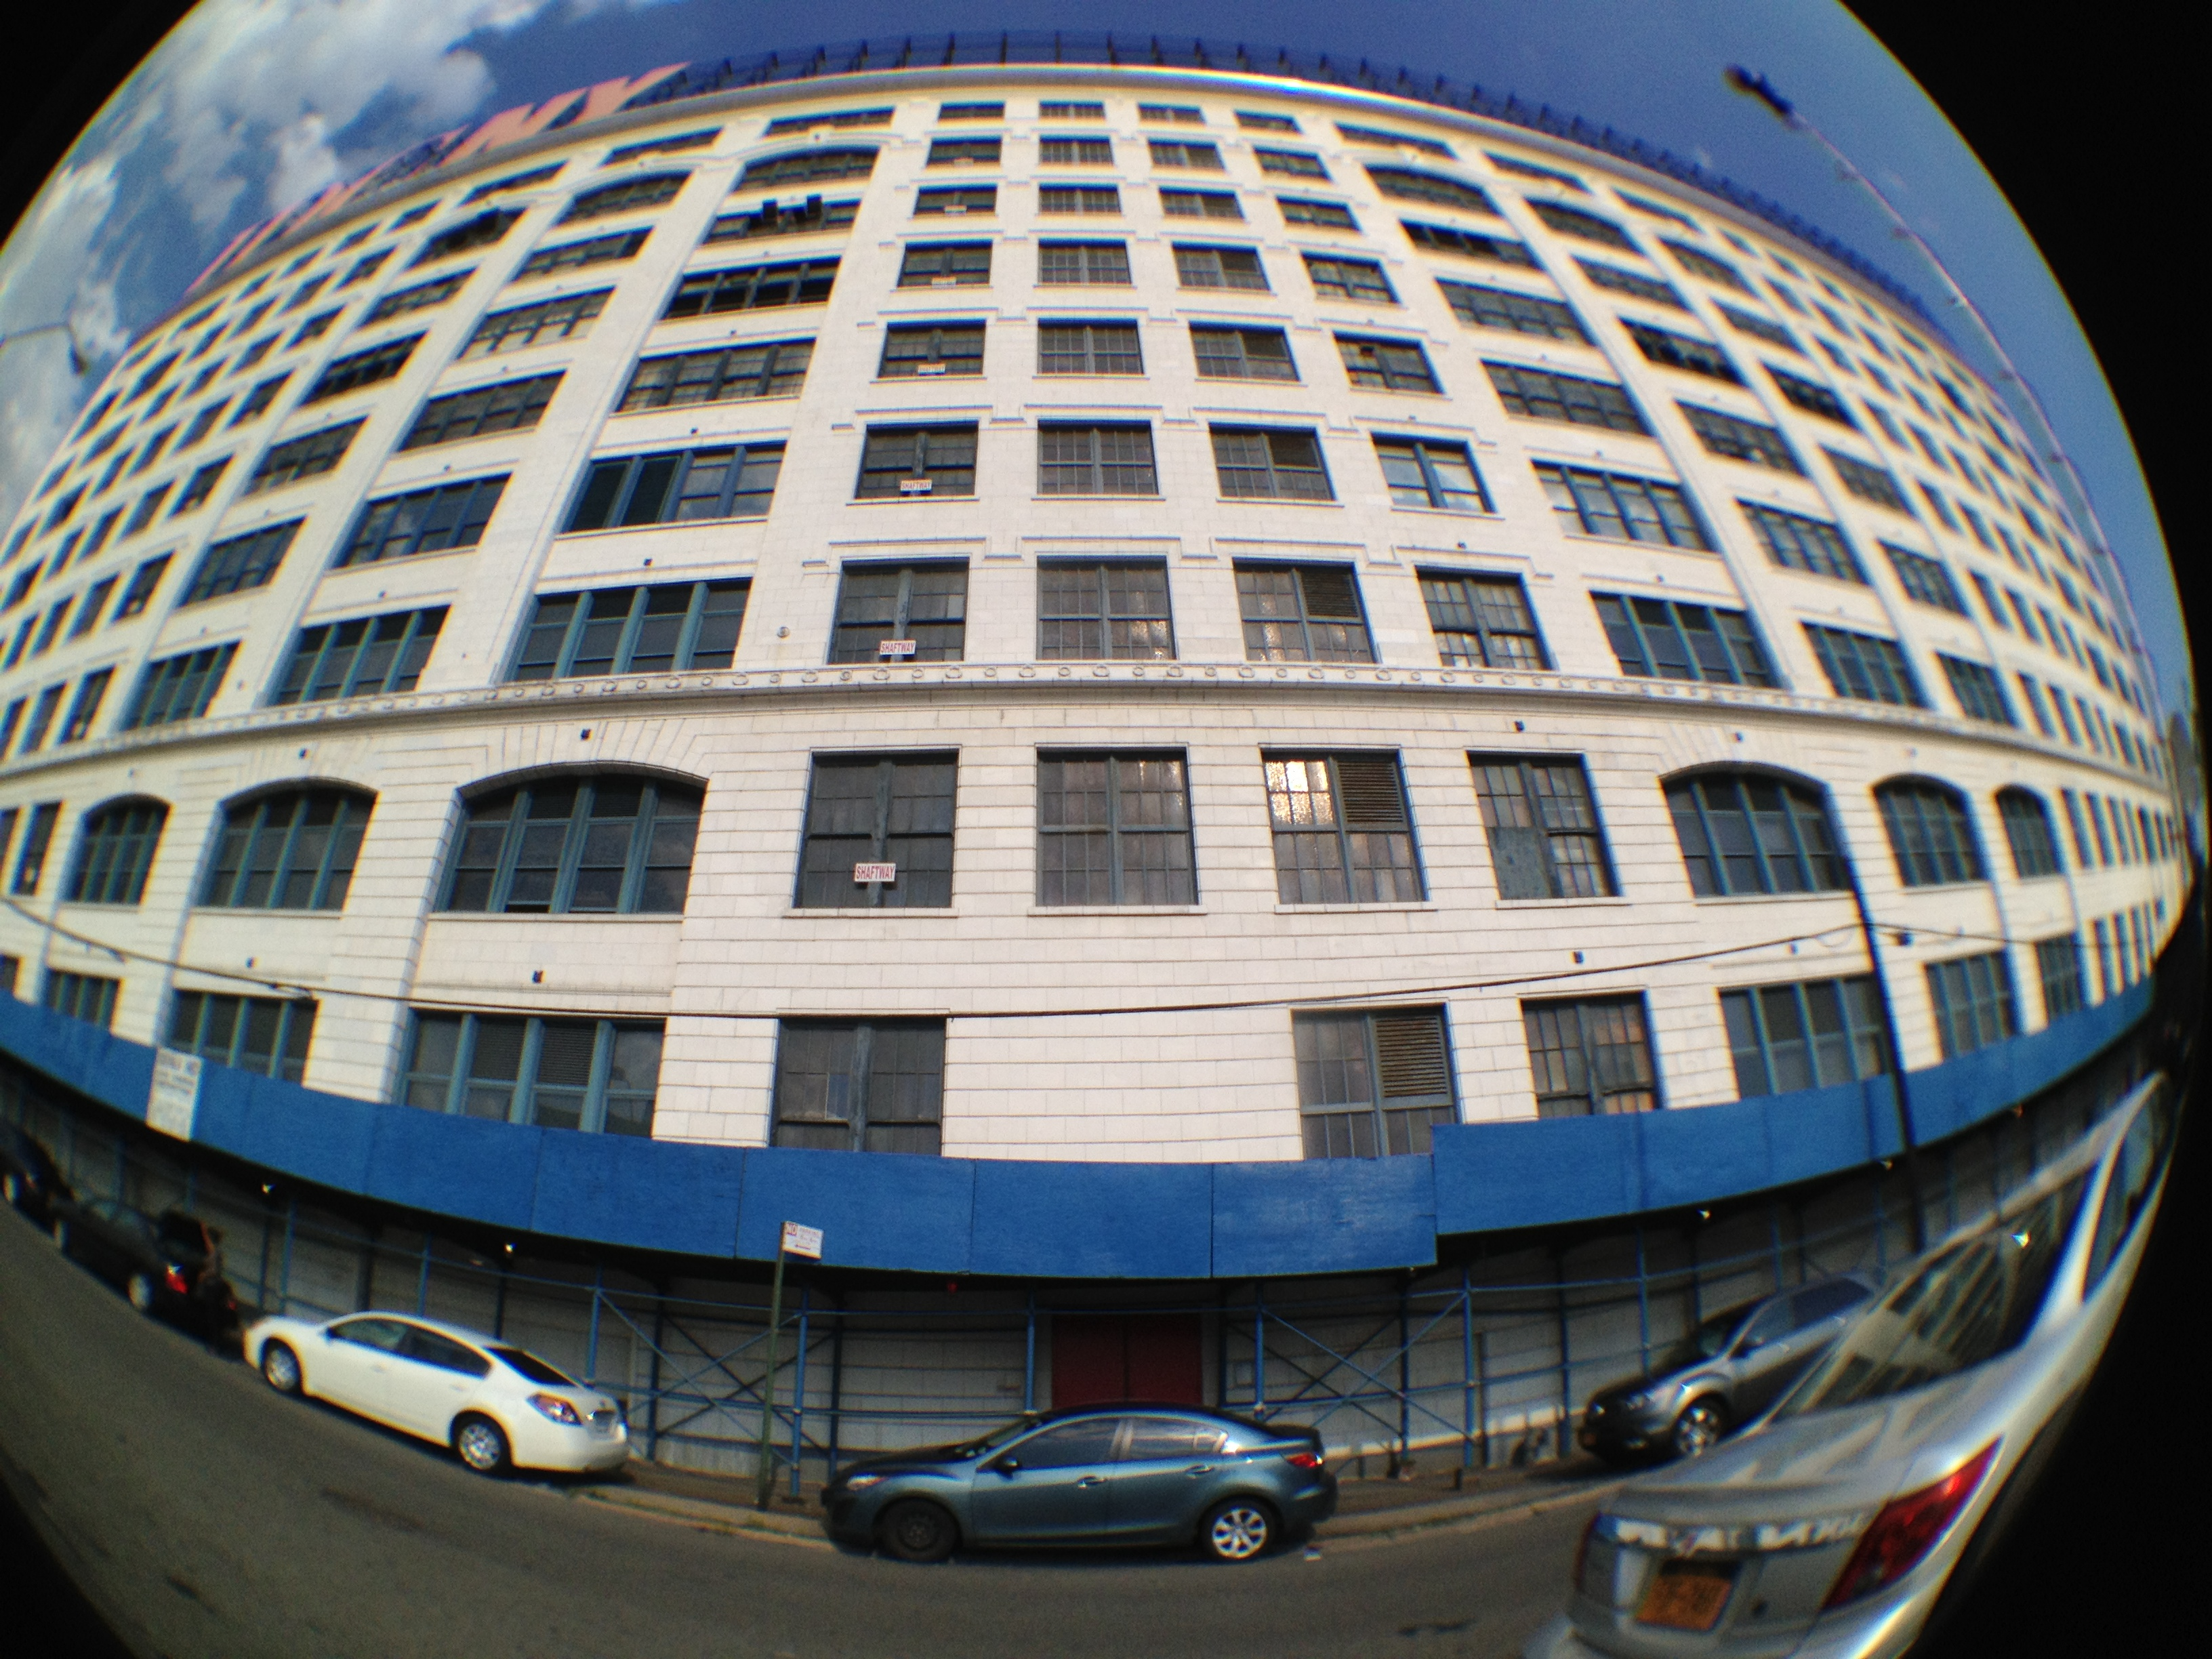
\includegraphics[width=0.65\textwidth]{fisheye}

    \caption{Barrel distortion in fish eye lens}
    \label{fig:fisheye}

\end{figure}

\subsection{Point filtering}

Not all points are eligible for the color registration, based on it's location and camera properties, so two filtering steps were used: the first filter removes the points outside the view frustum and the second removes the hidden points.

\subsubsection{View Frustrum Removal Filter}

The view frustum is defined as the region of space that is captured by the camera sensor, which for pinhole cameras is a pyramid truncated by two parallel planes (the near and far clipping planes), as seen in \cref{fig:visual-frustrum-3d}. The sides of the frustum are limited by the size of the sensor, so the points that lie outside the bounding box defined by the points $(0,0)$ and $(width, height)$ is excluded.


\begin{figure}[h]
    
    \tdplotsetmaincoords{70}{140}
    \centering
    \begin{tikzpicture}[tdplot_main_coords]
        \coordinate (eye) at (0,0,0);

        \node[above left, scale=0.7] at (eye) {eye point};

        \draw[thick,->] (eye) -- +(-10,0,0) node[anchor=north west]{$z$};
        \draw[thick,->] (eye) -- +(0,1,0) node[anchor=north west]{$x$};
        \draw[thick,->] (eye) -- +(0,0,-1) node[anchor=north]{$y$};

        \newcommand{\drawfrustumlines}[2]{
            \def\x{#1/#2};
            \draw[dashed] (eye) -- (#1, \x, \x);
            \draw[dashed] (eye) -- (#1, -\x, \x);
            \draw[dashed] (eye) -- (#1, \x, -\x);
            \draw[dashed] (eye) -- (#1, -\x, -\x);
        }
        \newcommand{\drawfrustum}[3]{
            \def\a{#1/#3};
            \def\b{#2/#3};
            \draw (#1, \a, \a) -- (#1, -\a, \a) -- (#1, -\a, -\a) -- (#1, \a, -\a) --cycle;
            \draw (#2, \b, \b) -- (#2, -\b, \b) -- (#2, -\b, -\b) -- (#2, \b, -\b) --cycle;
            \draw (#1, \a, \a) -- (#2, \b, \b);
            \draw (#1, -\a, \a) -- (#2, -\b, \b);
            \draw (#1, -\a, -\a) -- (#2, -\b, -\b);
            \draw (#1, \a, -\a) -- (#2, \b, -\b);

        }

        \drawfrustumlines{-10}{8};
        \drawfrustum{-8}{-4}{8};

        \draw[dashed] (0,0,-1.5) -- (0,0, -2);
        \draw[dashed] (-4,0,-2) -- (-4, 0, -1);
        \draw[dashed] (-8,0,-2) -- (-8, 0, -1.5);

        \draw[latex-latex] (0,0,-2) -- (-4, 0, -2) node[above, midway, sloped] {$z_{near}$};
        \draw[-latex] (-4,0,-2) -- (-8, 0, -2) node[above, midway, sloped] {$z_{far}$};
        
    \end{tikzpicture}

    \caption{Representation of the visual frustum of the camera}
    \label{fig:visual-frustrum-3d}

\end{figure}

The near and far clipping planes should reject the points based on the depth of field of the camera. The depth of field, or DOF, is the distance from the camera to the objects range, so that this objects are in focus. If the object falls out of this range, it starts to loose focus incrementally the farther out it is. There is a point where the object is sharper, which is called point of optimal focus. Two factor influences the DOP: the aperture size and the focal length. The aperture influences the amplitude of the DOF, so a bigger aperture results in a narrower DOF, and the focal length defines the point of optimal focus, so a bigger focal length moves the DOF farther away from the camera. The near and far clipping plane should defined to be the boundaries of the DOF, so that all points are in focus.

Based on the frustum of the camera defined above, the points that do not respect \cref{eqn:frustum-condition} should be rejected.

\begin{equation}
    \label{eqn:frustum-condition}
    \begin{aligned}
                 & 0        & < u & < width \\
        \wedge \ & 0        & < v & < height \\
        \wedge \ & z_{near} & < z & < z_{far} \\
    \end{aligned}
\end{equation}

\subsubsection{Hidden Point Removal Filter}

Not all points that lie on the frustum of the camera are seen by the camera, because some of this points are occluded by nearer objects, so they need to be removed. A fast and straightforward solution is to use the point cloud resulting from the same acquisition as the image, because the sensor are considered close together. However, this is not the best solution, as it would be better if the whole point cloud was used.

In \cite{katz07}, an simple and fast operator, the Hidden Point Removal, or HPR, determines the visibility of point sets, viewed from a given viewport. This method is easily implemented and has a asymptotic complexity of $O(n \log n)$, where $n$ is the number of points in the point cloud. Moreover, this method work well for both sparse and dense point clouds.

The HPR operator operates on a set of points $\mathcal{P} = \{p_i | i = 1 \dots n \}$, and the goal is to determine whether $p_i$ is visible from a viewpoint $\mathcal{C}$. In this application, $C$ is the origin of the point cloud. The algorithm consists of two steps: the inversion and the convex hull construction.

The inversion step maps each point $p_i$ along the ray from $\mathcal{C}$ to $p_i$, such that $|p_i|$ is monotonically decreasing. There are multiple ways to perform the inversion, but in \cite{katz07} the \emph{spherical flipping} was used. Spherical flipping reflects a point $p_i$ with respect to a sphere of radius $R$ to the new point $\hat{p_i}$ by applying the \cref{eqn:spherical-flipping}.

\begin{equation}
    \label{eqn:spherical-flipping}
    \hat{p_i} = p_i + 2 (R - |p_i|) \frac{p_i}{|p_i|}
\end{equation}

Afterwards, the convex hull of $\hat{\mathcal{P}} \bigcup \{\mathcal{C}\}$, where $\hat{\mathcal{P}}$ is the transformed point set and $\mathcal{C}$ is the center of the sphere, is computed. Finally, the points that lie in the complex hull are the visible points of the point set.

This algorithm only has a parameter, which is the radius $R$ of the sphere used for the spherical flipping, which influences the amount of false positives of the algorithm. In general, $R$ is determined based on the maximum point length $max(|p_i|)$ and a exponential factor $\alpha$, such that $R = max(|p_i|) \times 10^{\alpha}$. In this application, a factor of $\alpha = 3$ was adequate.

As an example, the HPR operator was used in the Stanford Bunny point cloud, as seen in \cref{fig:hpr-operator-bunny} and, as seen, \cref{fig:after-hpr} only presents the points that are visible, as opposed to \cref{fig:before-hpr}.

\begin{figure}[h]
    
    \centering
    \begin{subfigure}{0.5\textwidth}
        \centering
        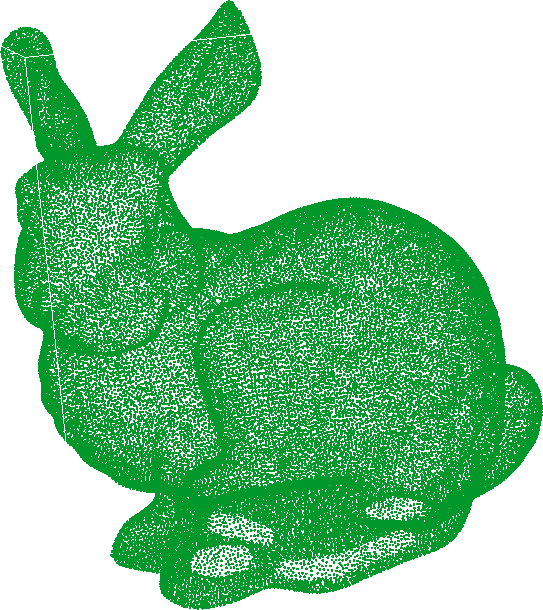
\includegraphics[height=6cm]{bunny-before-hpr}
        \caption{Before the HPR}
        \label{fig:before-hpr}
    \end{subfigure}%
    \begin{subfigure}{0.5\textwidth}
        \centering
        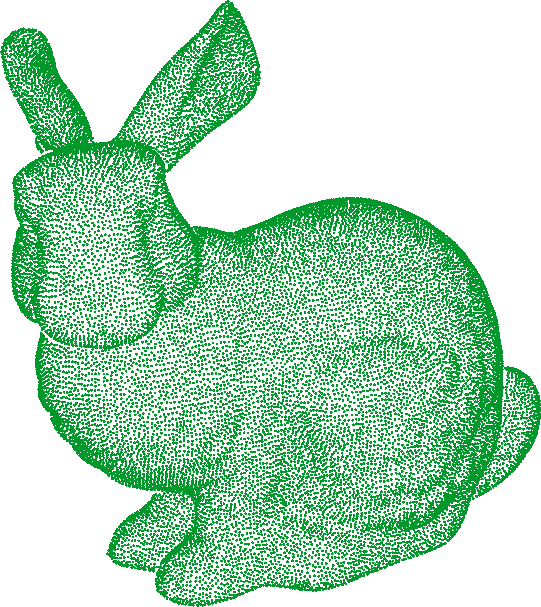
\includegraphics[height=6cm]{bunny-after-hpr}
        \caption{After the HPR}
        \label{fig:after-hpr}
    \end{subfigure}

    \caption{Result of the HPR operator in the Bunny point cloud}
    \label{fig:hpr-operator-bunny}

\end{figure}

\subsection{Color Attribution}

\newcommand\ceil[1]{\lceil #1 \rceil}
\newcommand\floor[1]{\lfloor #1 \rfloor}

Finally, the color is extracted from the image at the pixel coordinates $(u, v)$ and saved for the correspondent pixel. Because images are discrete, the color is interpolated using a bilinear interpolation, which uses the neighbor pixels to interpolate the color $C$ at $(u, v)$ in an image $I$ according to \cref{eqn:bilinear-interpolation} (the ceil and floor operators are, respectively, $\ceil{\cdot}$ and $\floor{\cdot}$). The interpolation can be visualized in \cref{fig:bilinear-interpolation}.

\begin{equation}
    \label{eqn:bilinear-interpolation}
    \begin{aligned}
        C(u, v) = \ & (u - \ceil{u}) \ (v - \ceil{v}) \ I_{\floor{u}, \floor{v}} \\
                + \ &  (u - \ceil{u}) \ (v - \floor{v}) \ I_{\floor{u}, \ceil{v}} \\
                + \ &  (u - \floor{u}) \ (v - \ceil{v}) \ I_{\ceil{u}, \floor{v}} \\
                + \ &  (u - \floor{u}) \ (v - \floor{v}) \ I_{\ceil{u}, \ceil{v}} \\
    \end{aligned}
\end{equation}

\begin{figure}[h]
    \centering
    \begin{tikzpicture}
        \draw[-latex] (-1, -1) -- (4, -1) node[below] {$u$};
        \draw[-latex] (-1, -1) -- (-1, 4) node[left] {$v$};

        \coordinate (c00) at (0,0);
        \coordinate (c10) at (3,0);
        \coordinate (c01) at (0,3);
        \coordinate (c11) at (3,3);
        \coordinate (c) at (1.7, 1.7);

        \draw[fill] (c00) circle (0.04) node[above right, scale=0.7] {$(\floor{u}, \floor{v})$};
        \draw[fill] (c10) circle (0.04) node[above right, scale=0.7] {$(\ceil{u}, \floor{v})$};
        \draw[fill] (c01) circle (0.04) node[above right, scale=0.7] {$(\floor{u}, \ceil{v})$};
        \draw[fill] (c11) circle (0.04) node[above right, scale=0.7] {$(\ceil{u}, \ceil{v})$};

        \draw[fill] (c) circle (0.04) node[above right, scale=0.7] {$(u, v)$};

        \draw[dotted] (c00) -- (c10) -- (c11) -- (c01) -- cycle;

        \draw[dotted] (c00) -| (c) -| cycle;

    \end{tikzpicture}

    \caption{Bilinear interpolation in an image}
    \label{fig:bilinear-interpolation}

\end{figure}
